\documentclass[conference,a4paper]{IEEEtran}
\usepackage{booktabs}
\usepackage{cite}
\usepackage{amsmath}
\usepackage{tikz}
\usetikzlibrary{positioning,arrows.meta,calc}
\begin{document}

\title{Patient-Conditioned Graph Learning for Organ-Level Adverse Drug Event Prediction from Spontaneous Reports}
\author{\IEEEauthorblockN{[Author names]}
\IEEEauthorblockA{[Affiliation, city, country]\\ {[email]}}}
\maketitle

\begin{abstract}
Clinicians cannot memorize every molecular target of every drug, and the organ-level consequences of a prescription may depend on the patient. We study a first step toward a patient digital twin: predicting which of eight organ systems appear in an adverse event report, given a drug and basic patient attributes. We combine 309,424 FDA Adverse Event Reporting System (FAERS) reports from 2025 with a drug--gene--organ graph built from ChEMBL mechanisms and curated Comparative Toxicogenomics Database associations. On a temporal split, a drug-identity model with patient features performs best (macro AUROC 0.732), exceeding a per-drug frequency baseline (0.711) and matching gradient boosting on patient, drug-class and chemical-fingerprint features (0.731); the graph does not help drugs seen in training. On drugs held out from training, the graph-and-patient model reaches 0.643, against 0.583 for patient features alone and 0.625 for gradient boosting, and leads both in all ten held-out splits. Ablations show that this gain depends on correct target edges: shuffling drug--target links lowers AUROC to 0.567, below patient features alone, while drug class alone recovers about two-thirds of the gain. Discrimination among patients taking the same drug remains modest (0.57--0.59). The results support mechanism graphs for drugs without report history, but do not support individual-level clinical use.
\end{abstract}

\begin{IEEEkeywords}
adverse drug events, digital twin, graph neural networks, pharmacovigilance, eHealth
\end{IEEEkeywords}

\section{Introduction}
A drug can act on many targets, and those targets can be linked to several organ systems. Tracing these links by hand is impractical during routine prescribing. A patient digital twin, a computational model of an individual patient~\cite{bjornsson2020,katsoulakis2024}, could support this reasoning by estimating which organ systems deserve attention for a given patient and drug.

Graph learning has been applied to polypharmacy side effects~\cite{zitnik2018} and drug repurposing~\cite{huang2024}, and spontaneous reports have long supported signal detection~\cite{tatonetti2012}. We ask a narrower question: how much do mechanism knowledge and patient attributes each contribute to organ-level prediction, and when?

Our contributions are: (1) a reproducible pipeline linking FAERS reports to a drug--gene--organ graph; (2) a controlled comparison separating the effects of drug identity, graph structure and patient attributes on seen and unseen drugs, including classical comparators that use chemical structure; (3) graph ablations that identify which part of the mechanism knowledge carries the gain on unseen drugs; and (4) a within-drug metric that measures patient-level discrimination, which aggregate scores can conceal.

\section{Related Work}
Decagon modeled polypharmacy side effects as link prediction on a multimodal graph of drugs and proteins~\cite{zitnik2018}. TxGNN used a medical knowledge graph for zero-shot drug repurposing~\cite{huang2024}. Tatonetti \emph{et al.} used adverse event reports to study drug effects and interactions while addressing confounding~\cite{tatonetti2012}. Side-effect profiles have been predicted from chemical fragments~\cite{pauwels2011}, from combined chemical, biological and phenotypic properties~\cite{liu2012}, and, for side-effect frequencies, by matrix decomposition~\cite{galeano2020}, mostly using label-derived resources such as SIDER~\cite{kuhn2016}. Bean \emph{et al.} built a knowledge graph of drugs, targets, indications and adverse reactions and validated its predictions in electronic health records~\cite{bean2017}. These studies predict drug-level profiles. Our focus differs: we separate drug history, mechanism structure and patient attributes at the organ level, including among patients taking the same drug. We do not claim a new graph architecture; our contribution is the controlled evaluation.

\section{Data}
\textbf{Reports.} We used the four 2025 FAERS quarterly files. We kept the latest version of each case, as is standard for FAERS~\cite{sakaeda2013}, and matched the primary suspect ingredient to ChEMBL approved small molecules~\cite{zdrazil2024} after removing common salt terms. Of 1,469,305 cases, 695,719 matched a drug, and 309,424 had at least one organ-mapped event, covering 1,167 drugs. Patient inputs were age, sex, weight, missingness indicators and the number of other reported drugs. Among the 78,880 fourth-quarter test reports, age was present in 70.3\% and weight in 25.9\% (61.6\% and 16.8\% in the full quarterly file).

\textbf{Labels.} Reported MedDRA preferred terms~\cite{brown1999} were mapped by a transparent keyword list to eight systems: liver, heart, nervous, kidney, lung, gastrointestinal, skin and blood. Table~\ref{tab:data} lists report counts and label prevalence. Only 26.3\% of event rows mapped to an organ, because many terms, such as ``Off label use'' and ``Drug ineffective'', do not describe an organ.

\begin{table}[t]
\centering
\caption{Dataset summary after filtering.}
\label{tab:data}
\begin{tabular}{lrlr}
\toprule
Quarter & Reports & Organ label & Prevalence \\
\midrule
2025 Q1 & 72,430 & Liver & 9.9\% \\
2025 Q2 & 72,841 & Heart & 14.5\% \\
2025 Q3 & 85,273 & Nervous & 25.7\% \\
2025 Q4 & 78,880 & Kidney & 9.8\% \\
 & & Lung & 23.3\% \\
 & & Gastrointestinal & 29.7\% \\
 & & Skin & 18.0\% \\
 & & Blood & 10.6\% \\
\bottomrule
\end{tabular}
\end{table}

\textbf{Graph.} The graph has drug, gene and organ nodes. ChEMBL mechanisms give 4,716 drug--gene edges over 1,363 drugs, restricted to human targets. Curated CTD gene--disease associations~\cite{davis2023}, mapped with the same keyword list, give 6,533 gene--organ edges. The graph has 4,800 genes, and 86.8\% of reports involve a drug with at least one target.

\section{Methods}
\begin{figure*}[t]
\centering
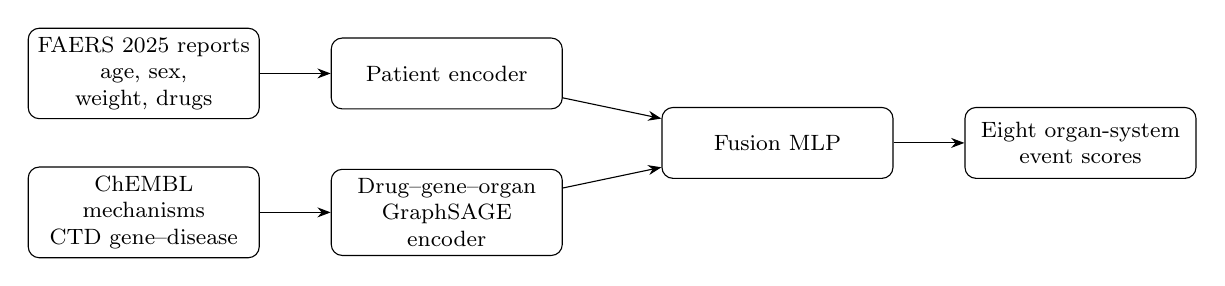
\begin{tikzpicture}[font=\footnotesize, node distance=6mm and 9mm, box/.style={draw, rounded corners, align=center, minimum height=9mm, text width=27mm}, >={Stealth}]
\node[box] (f) {FAERS 2025 reports\\age, sex, weight, drugs};
\node[box, below=of f] (c) {ChEMBL mechanisms\\CTD gene--disease};
\node[box, right=of f] (p) {Patient encoder};
\node[box, right=of c] (g) {Drug--gene--organ\\GraphSAGE encoder};
\node[box] (h) at ($(p)!0.5!(g)+(42mm,0)$) {Fusion MLP};
\node[box, right=of h] (o) {Eight organ-system\\event scores};
\draw[->] (f) -- (p);
\draw[->] (c) -- (g);
\draw[->] (p) -- (h);
\draw[->] (g) -- (h);
\draw[->] (h) -- (o);
\end{tikzpicture}
\caption{Overview of the pipeline. Patient attributes and mechanism knowledge are encoded separately, then combined to score organ systems for a report.}
\label{fig:pipe}
\end{figure*}

\textbf{Model.} Fig.~\ref{fig:pipe} summarizes the system. A two-layer heterogeneous GraphSAGE encoder~\cite{hamilton2017} produces a drug embedding $h_d$ from first-level ATC features and learned gene and organ embeddings. For each relation $r$, a layer aggregates neighbors and sums over relations:
\begin{equation}
h_v^{(l+1)} = \sigma\Big(\sum_{r} \mathrm{SAGE}_r\big(h_v^{(l)}, \{h_u^{(l)} : u \in \mathcal{N}_r(v)\}\big)\Big).
\end{equation}
A patient encoder maps the seven patient inputs $x$ to a 64-dimensional vector $z=f(x)$. A multilayer perceptron then gives organ probabilities,
\begin{equation}
\hat{y} = \mathrm{sigmoid}\big(g([h_d; z])\big) \in [0,1]^8,
\end{equation}
trained with binary cross-entropy over the eight organ labels. Because $h_d$ is computed from target neighbors and ATC features, the encoder can represent a drug with no training reports.

\textbf{Neural comparators.} We compare a global label rate, per-drug training frequency, patient features only, a learned drug-identity embedding with and without patient features, and the graph encoder with and without patient features.

\textbf{Classical comparators.} Logistic regression and histogram gradient boosting are trained per organ on the patient inputs, the first-level ATC vector and a 256-dimensional Morgan count fingerprint (radius 2)~\cite{rogers2010} of the drug. A structure $k$-nearest-neighbor model scores a test drug by the organ rates of its ten most similar training drugs, weighted by Tanimoto similarity of 1024-bit Morgan fingerprints. These comparators see chemical structure, which the graph model does not.

\textbf{Ablations.} To test which part of the graph carries the signal, we retrain the graph-and-patient model with (i) the ATC input replaced by a constant, (ii) all drug--target edges removed, leaving ATC class as the only drug input, and (iii) the gene endpoints of drug--target edges randomly permuted, so that each drug keeps its number of targets but not their identity.

\textbf{Evaluation.} The temporal split trains on the first three quarters and tests on the fourth. The cold-drug split holds out 20\% of drugs with graph targets, removing all of their reports from training while keeping their target edges. Identity models are excluded from this split because unseen drugs have untrained embeddings. Each setting uses ten seeds, which vary initialization and the validation sample; the cold-drug split also draws a new set of held-out drugs per seed. All models share the same splits per seed. We report macro AUROC and AUPRC over organs. Within-drug AUROC is computed separately for drugs with at least 200 test reports and for organs with at least 20 positive and 20 negative reports in that drug, then averaged. Models without patient inputs score 0.5 by construction, so any gain reflects differences among patients on the same drug. Training used AdamW, early stopping on a 10\% validation sample and one RTX 5070 Ti Laptop GPU.

\section{Results}
\begin{table}[t]
\centering
\caption{Test performance, mean $\pm$ SD over ten seeds.}
\label{tab:main}
\footnotesize
\setlength{\tabcolsep}{2pt}
\begin{tabular}{llccc}
\toprule
Split & Model & AUROC & AUPRC & Within-drug \\
\midrule
Temporal & Global rate & .500 $\pm$ .001 & .181 $\pm$ .000 & .500 \\
 & Drug frequency & .711 $\pm$ .000 & .367 $\pm$ .000 & .500 \\
 & Patient only & .592 $\pm$ .000 & .258 $\pm$ .001 & .568 $\pm$ .001 \\
 & Logistic regression & .702 $\pm$ .000 & .350 $\pm$ .000 & .566 $\pm$ .000 \\
 & Gradient boosting & .731 $\pm$ .000 & \textbf{.400} $\pm$ .000 & \textbf{.592} $\pm$ .001 \\
 & Structure $k$-NN & .650 $\pm$ .000 & .293 $\pm$ .000 & .500 \\
 & Drug ID & .710 $\pm$ .001 & .368 $\pm$ .001 & .500 \\
 & Drug ID + patient & \textbf{.732} $\pm$ .000 & .397 $\pm$ .000 & .588 $\pm$ .001 \\
 & Graph & .694 $\pm$ .000 & .345 $\pm$ .001 & .500 $\pm$ .001 \\
 & Graph + patient & .720 $\pm$ .001 & .380 $\pm$ .001 & .585 $\pm$ .001 \\
\midrule
Cold drug & Global rate & .501 $\pm$ .001 & .177 $\pm$ .003 & .500 \\
 & Patient only & .583 $\pm$ .009 & .248 $\pm$ .015 & .578 $\pm$ .005 \\
 & Logistic regression & .577 $\pm$ .011 & .223 $\pm$ .012 & .579 $\pm$ .004 \\
 & Gradient boosting & .625 $\pm$ .020 & .279 $\pm$ .019 & .580 $\pm$ .006 \\
 & Structure $k$-NN & .558 $\pm$ .018 & .216 $\pm$ .016 & .500 \\
 & Graph & .609 $\pm$ .015 & .251 $\pm$ .013 & .500 \\
 & Graph + patient & \textbf{.643} $\pm$ .016 & \textbf{.287} $\pm$ .017 & \textbf{.584} $\pm$ .005 \\
\bottomrule
\end{tabular}
\end{table}

Table~\ref{tab:main} gives the main results. Differences below are paired by seed and reported as mean with a 95\% interval across seeds. Seeds share most of their data, so these intervals describe variation across training runs and held-out drug sets rather than sampling uncertainty for a new population; we read them as evidence of a consistent direction.

On the temporal split, adding patient features to drug identity improved AUROC over per-drug frequency by 0.021 (0.020--0.021), in all ten seeds. Gradient boosting came within 0.001 of this model and had the best AUPRC and within-drug AUROC. Its fingerprints identify each seen drug, so it has access to the same report history. The graph model with patient features was 0.012 below the identity model in every seed, so mechanism structure gave no benefit when a drug already had report history.

On unseen drugs the pattern changed. Graph plus patient features exceeded patient features alone by 0.060 (0.050--0.070) and the graph alone by 0.034 (0.024--0.044). It also exceeded gradient boosting by 0.018 (0.011--0.024), logistic regression by 0.066 and structure $k$-NN by 0.085. Every one of these differences was positive in all ten seeds. Chemical similarity alone was a weak predictor of organ profile on unseen drugs.

\begin{table}[t]
\centering
\caption{Graph ablations of the graph-and-patient model (ten seeds). $\Delta$: paired cold-drug AUROC difference from the full model, with 95\% interval across seeds. Without target edges, ATC class is the only drug input.}
\label{tab:abl}
\footnotesize
\setlength{\tabcolsep}{2.5pt}
\begin{tabular}{lccc}
\toprule
 & Temporal & \multicolumn{2}{c}{Cold drug} \\
Variant & AUROC & AUROC & $\Delta$ \\
\midrule
Full & .720 & .643 $\pm$ .016 & -- \\
No ATC input & .709 & .644 $\pm$ .018 & $+$.001 ($-$.004, .006) \\
No target edges & .651 & .623 $\pm$ .011 & $-$.020 ($-$.026, $-$.013) \\
Shuffled targets & .721 & .567 $\pm$ .011 & $-$.076 ($-$.090, $-$.063) \\
Patient only & .592 & .583 $\pm$ .009 & $-$.060 ($-$.070, $-$.050) \\
\bottomrule
\end{tabular}
\end{table}

Table~\ref{tab:abl} shows where the gain on unseen drugs comes from. Shuffling the gene endpoints of target edges lowered cold-drug AUROC by 0.076, to below the patient-only model in nine of ten seeds, so incorrect targets mislead the model rather than simply adding noise. ATC class without target edges reached 0.623, recovering 0.040 of the 0.060 gain over patient features alone; adding the true targets raised it by a further 0.020, in nine of ten seeds. Removing the ATC input had no measurable effect when target edges were present, which suggests that the targets already carry the class information. On the temporal split, shuffled edges matched the full model (difference 0.001), consistent with the graph acting mainly as a drug identifier when report history exists.

Within-drug AUROC stayed between 0.57 and 0.59 for every model with patient inputs. The patient-only model already reached 0.568 on the temporal split, so most of this signal comes from the attributes themselves.

Table~\ref{tab:organ} shows that performance varies by organ. With report history, blood and liver events were easiest to rank and gastrointestinal events hardest. On unseen drugs, the graph gave its largest gains over patient features for kidney (+0.085), blood (+0.082) and nervous system events (+0.078), and its smallest for heart events (+0.036). It exceeded gradient boosting for every organ except heart ($-$0.003). Seeds 0--4 were also run in an earlier five-seed experiment; mean AUROC of each graph model changed by at most 0.001 and single-seed values by less than 0.006, and reported values come from the final ten-seed run.

\begin{table}[t]
\centering
\caption{Mean AUROC by organ system over ten seeds. GB: gradient boosting; pat.: patient features.}
\label{tab:organ}
\footnotesize
\setlength{\tabcolsep}{3pt}
\begin{tabular}{lcccc}
\toprule
 & Temporal & \multicolumn{3}{c}{Cold drug} \\
Organ & ID + pat. & Patient & GB & Graph + pat. \\
\midrule
Liver & .775 & .610 & .629 & .659 \\
Heart & .710 & .575 & .614 & .611 \\
Nervous & .696 & .558 & .619 & .636 \\
Kidney & .744 & .586 & .649 & .671 \\
Lung & .725 & .588 & .618 & .631 \\
Gastrointestinal & .685 & .574 & .591 & .613 \\
Skin & .713 & .573 & .633 & .639 \\
Blood & .805 & .601 & .650 & .683 \\
\bottomrule
\end{tabular}
\end{table}

\section{Discussion and Limitations}
The practical finding is conditional: report history is the stronger signal for established drugs, while mechanism knowledge helps when that history is absent. The ablations sharpen this claim: the gain on unseen drugs depends on correct drug--target links, and drug class explains part but not all of it. This is relevant to newly marketed drugs, although our held-out drugs are approved drugs with existing mechanism annotations. A fingerprint-based comparator that sees chemical structure still trailed the graph model, so combining structure and mechanism inputs is a natural next step.

These results describe patterns in reports, not risk. FAERS is voluntary, has no exposure denominator, and cannot establish causality. Reports are subject to under-reporting and stimulated reporting, and patient attributes may act as proxies for the indication. We condition on reports with at least one organ-mapped event, so outputs are not incidence estimates. Keyword labels are an approximation of standardized MedDRA grouping and were not reviewed by clinicians. Patient inputs omit laboratory values, comorbidities, dose and genotype, and weight is largely missing. Only the primary suspect drug is modeled, so drug--drug interactions are not addressed. The temporal test set is fixed, so its small standard deviations reflect training variation only. The edge shuffle preserves each drug's number of targets but not each gene's degree, and all ablations use a single architecture.

The current system is therefore a research prototype and must not guide treatment. Within-drug performance of 0.57--0.59 is far from what individual decisions would require.

\section{Conclusion}
We linked real adverse event reports to a mechanism graph and separated what each information source contributes. Patient attributes gave a small, consistent gain. On drugs excluded from training, the graph outperformed patient-only, chemical-structure and fingerprint-boosting comparators in every seed, and this advantage disappeared when target links were shuffled. Future work should validate these findings on longitudinal clinical records with laboratory values, standardized MedDRA labels and clinician review.

\begin{thebibliography}{99}
\bibitem{bjornsson2020} B. Bj\"{o}rnsson \emph{et al.}, ``Digital twins to personalize medicine,'' \emph{Genome Medicine}, vol. 12, art. no. 4, 2020, doi: 10.1186/s13073-019-0701-3.
\bibitem{katsoulakis2024} E. Katsoulakis \emph{et al.}, ``Digital twins for health: a scoping review,'' \emph{npj Digital Medicine}, vol. 7, art. no. 77, 2024, doi: 10.1038/s41746-024-01073-0.
\bibitem{zitnik2018} M. Zitnik, M. Agrawal, and J. Leskovec, ``Modeling polypharmacy side effects with graph convolutional networks,'' \emph{Bioinformatics}, vol. 34, no. 13, pp. i457--i466, 2018.
\bibitem{huang2024} K. Huang \emph{et al.}, ``A foundation model for clinician-centered drug repurposing,'' \emph{Nature Medicine}, 2024, doi: 10.1038/s41591-024-03233-x.
\bibitem{tatonetti2012} N. P. Tatonetti, P. P. Ye, R. Daneshjou, and R. B. Altman, ``Data-driven prediction of drug effects and interactions,'' \emph{Science Translational Medicine}, vol. 4, no. 125, 2012.
\bibitem{pauwels2011} E. Pauwels, V. Stoven, and Y. Yamanishi, ``Predicting drug side-effect profiles: a chemical fragment-based approach,'' \emph{BMC Bioinformatics}, vol. 12, art. no. 169, 2011, doi: 10.1186/1471-2105-12-169.
\bibitem{liu2012} M. Liu \emph{et al.}, ``Large-scale prediction of adverse drug reactions using chemical, biological, and phenotypic properties of drugs,'' \emph{J. Am. Med. Inform. Assoc.}, vol. 19, no. e1, pp. e28--e35, 2012.
\bibitem{galeano2020} D. Galeano, S. Li, M. Gerstein, and A. Paccanaro, ``Predicting the frequencies of drug side effects,'' \emph{Nature Communications}, vol. 11, art. no. 4575, 2020, doi: 10.1038/s41467-020-18305-y.
\bibitem{kuhn2016} M. Kuhn, I. Letunic, L. J. Jensen, and P. Bork, ``The SIDER database of drugs and side effects,'' \emph{Nucleic Acids Research}, vol. 44, no. D1, pp. D1075--D1079, 2016.
\bibitem{bean2017} D. M. Bean \emph{et al.}, ``Knowledge graph prediction of unknown adverse drug reactions and validation in electronic health records,'' \emph{Scientific Reports}, vol. 7, art. no. 16416, 2017.
\bibitem{sakaeda2013} T. Sakaeda, A. Tamon, K. Kadoyama, and Y. Okuno, ``Data mining of the public version of the FDA Adverse Event Reporting System,'' \emph{Int. J. Med. Sci.}, vol. 10, no. 7, pp. 796--803, 2013.
\bibitem{zdrazil2024} B. Zdrazil \emph{et al.}, ``The ChEMBL Database in 2023: a drug discovery platform spanning multiple bioactivity data types and time periods,'' \emph{Nucleic Acids Research}, vol. 52, no. D1, pp. D1180--D1192, 2024.
\bibitem{brown1999} E. G. Brown, L. Wood, and S. Wood, ``The Medical Dictionary for Regulatory Activities (MedDRA),'' \emph{Drug Safety}, vol. 20, no. 2, pp. 109--117, 1999.
\bibitem{davis2023} A. P. Davis \emph{et al.}, ``Comparative Toxicogenomics Database (CTD): update 2023,'' \emph{Nucleic Acids Research}, vol. 51, no. D1, pp. D1257--D1262, 2023.
\bibitem{hamilton2017} W. Hamilton, Z. Ying, and J. Leskovec, ``Inductive representation learning on large graphs,'' in \emph{Advances in Neural Information Processing Systems}, 2017.
\bibitem{rogers2010} D. Rogers and M. Hahn, ``Extended-connectivity fingerprints,'' \emph{J. Chem. Inf. Model.}, vol. 50, no. 5, pp. 742--754, 2010.
\end{thebibliography}

\end{document}
